\beginsong{Bündische Vaganten}[wuw={trenk (Alo Hamm), 1952}, bo={178}, pfii={27}, pfiii={58}, index={Hej, wie vorn der Fetzen fliegt}]

\markboth{\songtitle}{\songtitle}

\beginverse
\endverse

\centering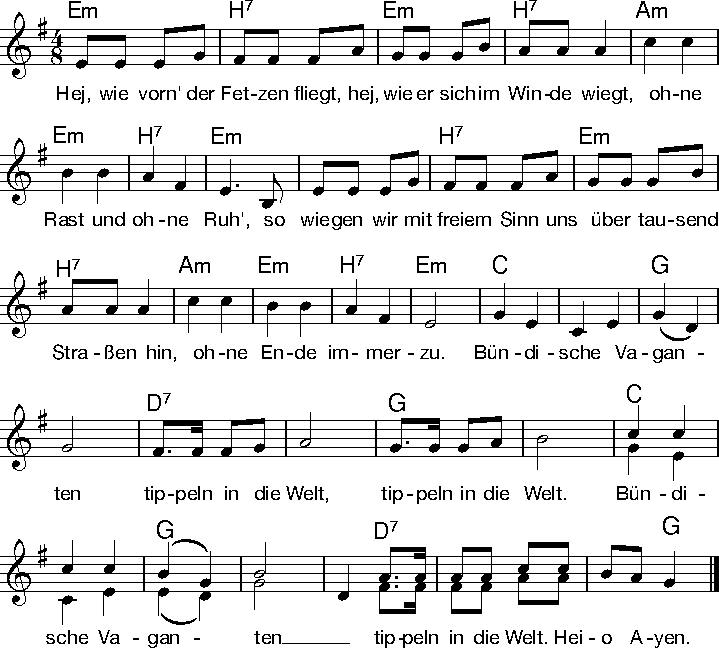
\includegraphics[width=1\textwidth]{Noten/Lied011.pdf}

\beginverse
\[Em]Treiben wir dem \[H7]Süden zu, lässt \[Em]uns der Norden \[H7]keine Ruh',
\[Am]über\[Em]all zu \[H7]Haus' sind \[Em]wir.
Mal \[Em]rüber nach A\[H7]merika, mal \[Em]runter bis nach \[H7]Afrika,
\[Am]hoja, \[Em]hoja, \[H7]das sind \[Em]wir!
\endverse

\beginchorus 
\[C]Bündische Va\[G]ganten
tip\[D7]peln in die Welt, tip\[G]peln in die Welt.
\[C]Bündische Va\[G]ganten 
tip\[D7]peln in die Welt, hei-o A\[G]yen!
\endchorus

\beginverse
^Hast du noch ein ^jung' Gesicht, so ^zage nicht und ^fack'le nicht, 
^frage ^niemals ^nach dem ^'Wie?'
Wer ^nur am Rand der ^Straße klebt, für ^seinen dummen ^Bauch nur lebt,
^misst der ^Ferne ^Zauber ^nie.
\endverse
%\renewcommand{\everychorus}{\textnote{\bf Refrain (wdh.)}}
\beginchorus 
\[C]Bündische Va\[G]ganten
tip\[D7]peln in die Welt, tip\[G]peln in die Welt.
\[C]Bündische Va\[G]ganten
tip\[D7]peln in die Welt, hei-o A\[G]yen!
\endchorus


\endsong

\beginscripture{}
Vagant = Fahrendes Volk/Herumziehender; Das Lied behandelt die deutsche Jugendbewegung zwischen 1919 und 1933, die aus dem Wandervogel entstand und die Hinwendung der städtischen bürgerlichen Jugend zum Naturleben meint.
\endscripture

\begin{intersong}

\end{intersong}